In this section we report the observed and expected upper limits 
correspoinding to 1.5~$\ifb$ LP2011 dataset. 

Figure~\ref{fig:limits_lp_cut} shows the upper limits for the cut-based analysis, 
with the results tabulated in Table~\ref{tab:limits_lp} 
and Table~\ref{tab:limits_lp_cut_splitflavor}. 
Figure~\ref{fig:limits_lp_shape} shows the upper limits for the multivariate based analysis, 
with the results tabulated in Table~\ref{tab:limits_lp} 
and Table~\ref{tab:limits_lp_shape_splitflavor}. 

%%%%%%%%%%%%%%%%%%%%%%%%%%%%%%
\begin{figure}[!htbp]
\centering
\subfigure[]{
\centering
\label{subfig:0j_sf}
%\includegraphics[width=0.48\textwidth]{lp_figures/limits_0j_sf_cut_ana_v6_1500pb_LP.pdf}
}
\subfigure[]{
\centering
\label{subfig:0j_of}
%\includegraphics[width=0.48\textwidth]{lp_figures/limits_0j_of_cut_ana_v6_1500pb_LP.pdf}
}
\subfigure[]{
\centering
\label{subfig:1j_sf}
%\includegraphics[width=0.48\textwidth]{lp_figures/limits_1j_sf_cut_ana_v6_1500pb_LP.pdf}
}
\subfigure[]{
\centering
\label{subfig:1j_of}
%\includegraphics[width=0.48\textwidth]{lp_figures/limits_1j_of_cut_ana_v6_1500pb_LP.pdf}
}
\subfigure[]{
\centering
\label{subfig:2j}
%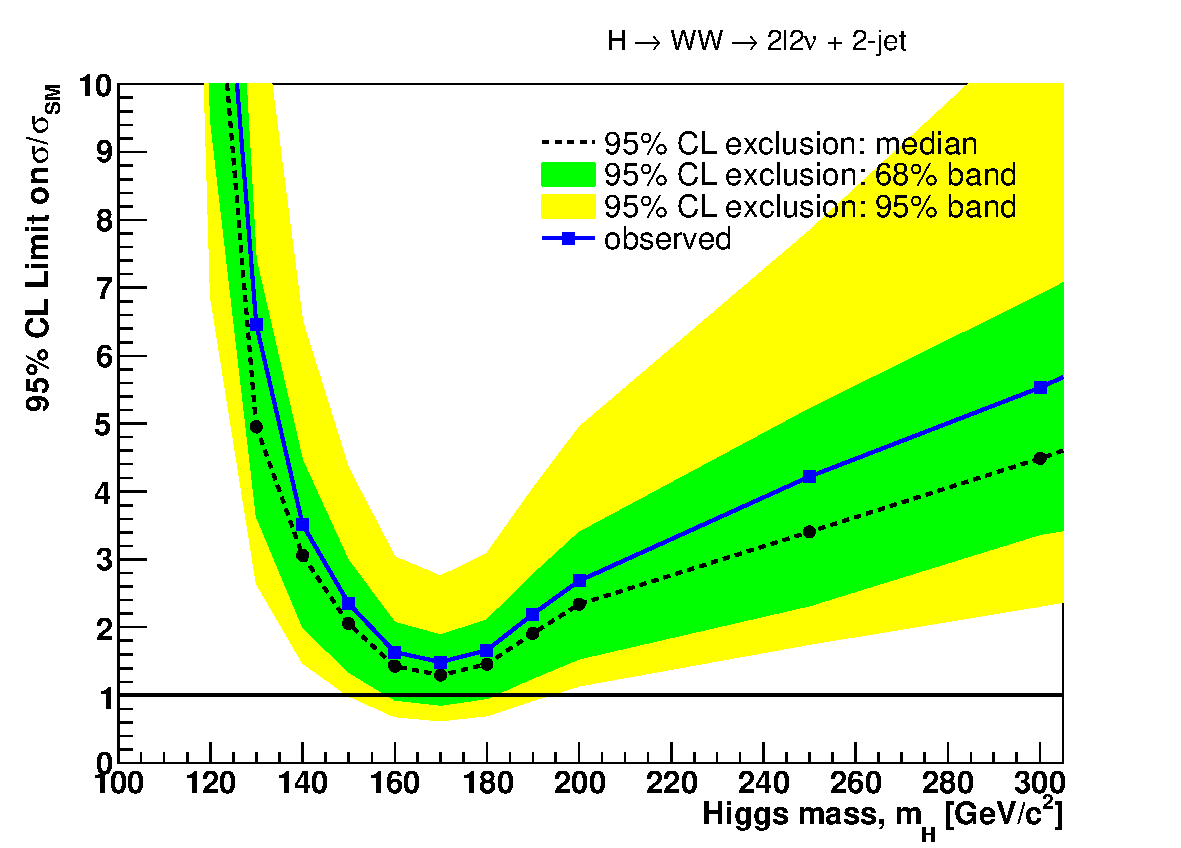
\includegraphics[width=0.48\textwidth]{lp_figures/limits_2j_cut_ana_v6_1500pb_LP.pdf}
}
\subfigure[]{
\centering
\label{subfig:nj}
%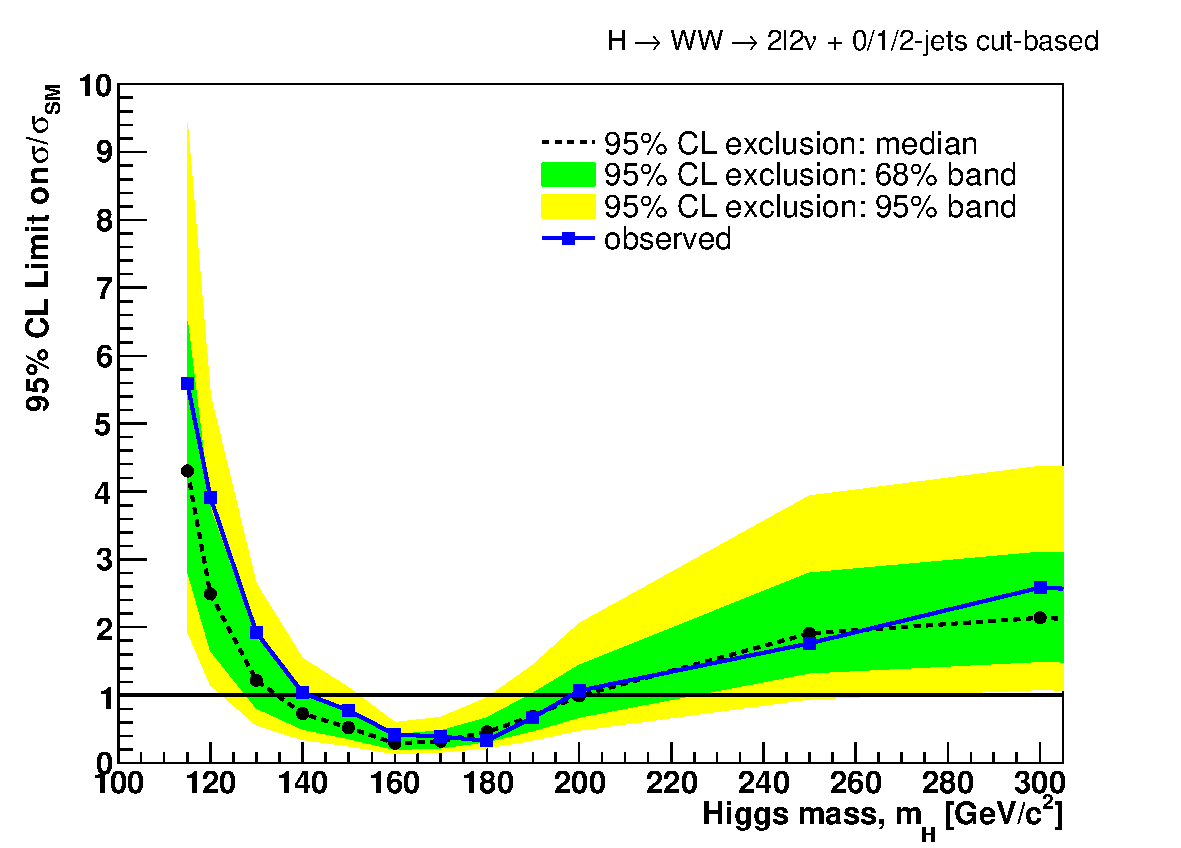
\includegraphics[width=0.48\textwidth]{lp_figures/limits_nj_cut_ana_v6_1500pb_LP.pdf}
}
\caption{Cut-based analysis upper limits at 95\% C.L. using data corresponding to 1.5~$\ifb$.
The limits are shown in 4 final states separately. \subref{subfig:0j_sf}: SF in 0 Jet bin; 
\subref{subfig:0j_of}: OF in 0 Jet bin; \subref{subfig:1j_sf}: SF in 1 Jet bin; 
\subref{subfig:1j_of}: OF in 1 Jet bin; \subref{subfig:2j}: 2 Jet bin; \subref{subfig:nj}: 0/1/2 Jets combined;
}
\label{fig:limits_lp_cut}
\end{figure}
%%%%%%%%%%%%%%%%%%%%%%%%%%%%%%


%%%%%%%%%%%%%%%%%%%%%%%%%%%%%%
\begin{figure}[!htbp]
\centering
\subfigure[]{
\centering
\label{subfig:0j_sf}
%\includegraphics[width=0.48\textwidth]{lp_figures/limits_0j_sf_shape_ana_v6_1500pb_LP_MTShape80.pdf}
}
\subfigure[]{
\centering
\label{subfig:0j_of}
%\includegraphics[width=0.48\textwidth]{lp_figures/limits_0j_of_shape_ana_v6_1500pb_LP_MTShape80.pdf}
}
\subfigure[]{
\centering
\label{subfig:1j_sf}
%\includegraphics[width=0.48\textwidth]{lp_figures/limits_1j_sf_shape_ana_v6_1500pb_LP_MTShape80.pdf}
}
\subfigure[]{
\centering
\label{subfig:1j_of}
%\includegraphics[width=0.48\textwidth]{lp_figures/limits_1j_of_shape_ana_v6_1500pb_LP_MTShape80.pdf}
}
\subfigure[]{
\centering
\label{subfig:nj}
%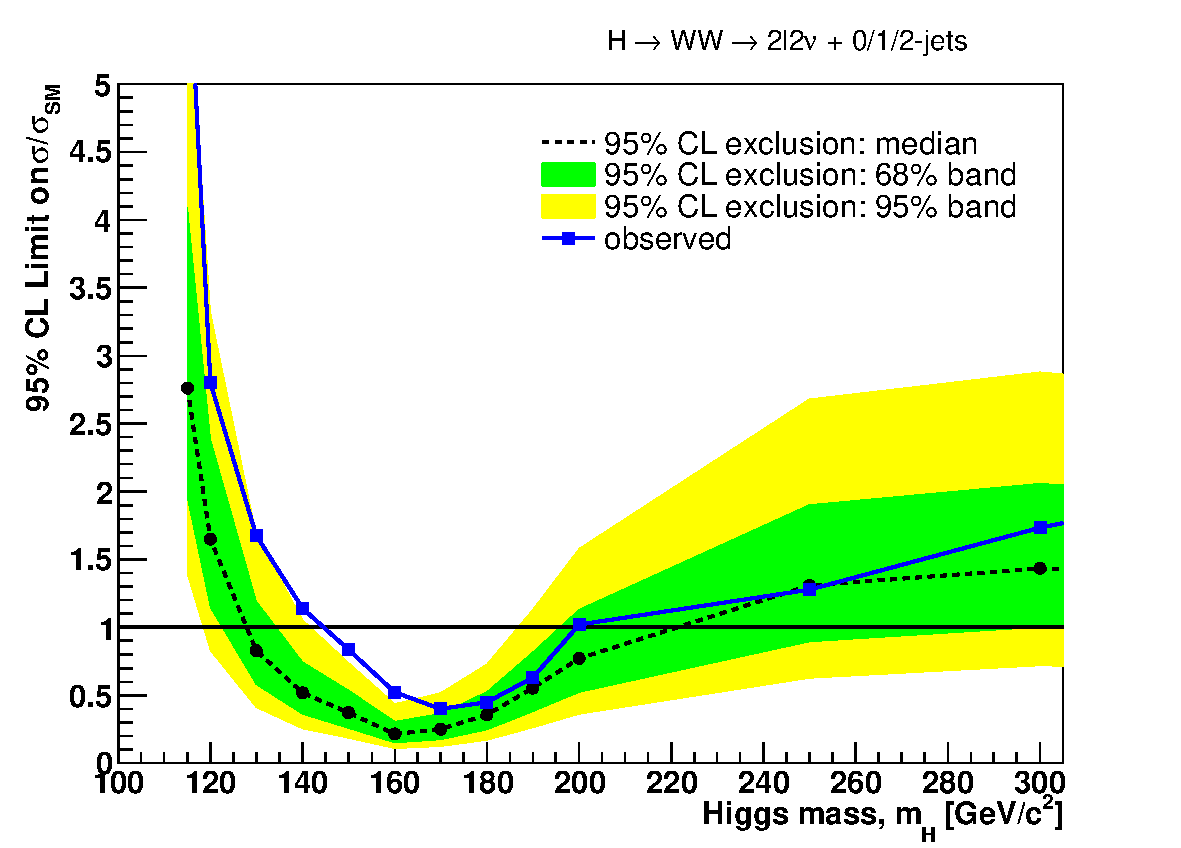
\includegraphics[width=0.48\textwidth]{lp_figures/limits_nj_shape_ana_v6_1500pb_LP.pdf}
}
\caption{Cut-based analysis upper limits at 95\% C.L. using data corresponding to 1.5~$\ifb$.
The limits are shown in 4 final states separately. \subref{subfig:0j_sf}: SF in 0 Jet bin; 
\subref{subfig:0j_of}: OF in 0 Jet bin; \subref{subfig:1j_sf}: SF in 1 Jet bin; 
\subref{subfig:1j_of}: OF in 1 Jet bin; \subref{subfig:2j}: 2 Jet bin; \subref{subfig:nj}: 0/1/2 Jets combined;
}
\label{fig:limits_lp_shape}
\end{figure}
%%%%%%%%%%%%%%%%%%%%%%%%%%%%%%
	
%%%%%%%%%%%%%%%%%%%%%%%%%%%%%%
\begin{table}
\begin{center}
\begin{tabular}{c c c c c}
\hline\hline
 $m_H$ (GeV) & Observed & Median Expected & 68\% C.L. Band & 95\% C.L. Band \\ \hline
\hline
\multicolumn{5}{c} {0/1/2-Jets Cut-Based}\\
\hline
% FIXME
\hline
\multicolumn{5}{c} {0/1/-Jets Multivariate Based combined with 2-Jet Cut Based}\\
\hline
% FIXME
\hline\hline
\end{tabular}
\end{center}
\caption{Upper limits at 95\% C.L. in 0, 1 and 2 Jet final states for both 
cut-based and multivariate based analyses, shown in Figure~\ref{fig:limits_lp_cut} 
and Figure~\ref{fig:limits_lp_shape}. 
The results correspond to the 1.5~$\ifb$ data 
} 
\label{tab:limits_lp}
\end{table}
%%%%%%%%%%%%%%%%%%%%%%%%%%%%%%



%%%%%%%%%%%%%%%%%%%%%%%%%%%%%%
\begin{table}
\begin{center}
\begin{tabular}{c c c c c}
\hline\hline
 $m_H$ (GeV) & Observed & Median Expected & 68\% C.L. Band & 95\% C.L. Band \\ \hline
\hline
\multicolumn{5}{c} {0-Jet Bin Same Flavor} \\
\hline
%FIXME
\hline
\multicolumn{5}{c} {0-Jet Bin Opposite Flavor} \\
\hline
%FIXME
\hline
\multicolumn{5}{c} {1-Jet Bin Same Flavor} \\
\hline
%FIXME
\hline
\multicolumn{5}{c} {1-Jet Bin Opposite Flavor} \\
\hline
%FIXME
\hline\hline
\end{tabular}
\end{center}
\caption{Cut based upper limits at 95\% C.L. in 0 and 1 Jet final state, 
using data corresponding to 1.5~$\ifb$ shown in 
Figure~\ref{fig:limits_lp_cut}.} 
\label{tab:limits_lp_cut_splitflavor}
\end{table}
%%%%%%%%%%%%%%%%%%%%%%%%%%%%%%

%%%%%%%%%%%%%%%%%%%%%%%%%%%%%%
\begin{table}
\begin{center}
\begin{tabular}{c c c c c}
\hline\hline
 $m_H$ (GeV) & Observed & Median Expected & 68\% C.L. Band & 95\% C.L. Band \\ \hline
\hline
\multicolumn{5}{c} {0-Jet Bin Same Flavor} \\
\hline
% FIXME
\hline
\multicolumn{5}{c} {0-Jet Bin Opposite Flavor} \\
\hline
% FIXME
\hline
\multicolumn{5}{c} {1-Jet Bin Same Flavor} \\
\hline
% FIXME
\hline
\multicolumn{5}{c} {1-Jet Bin Opposite Flavor} \\
\hline
% FIXME
\hline\hline
\end{tabular}
\end{center}
\caption{Multivariate based upper limits at 95\% C.L. in 0 and 1 Jet final state, 
using data corresponding to 1.5~$\ifb$ shown in 
Figure~\ref{fig:limits_lp_shape}.} 
\label{tab:limits_lp_shape_splitflavor}
\end{table}
%%%%%%%%%%%%%%%%%%%%%%%%%%%%%%
